\section{Results}\label{sec:results}

\subsection{Connected peers}\label{subsec:connected-peers}
\begin{figure*}[!ht]
    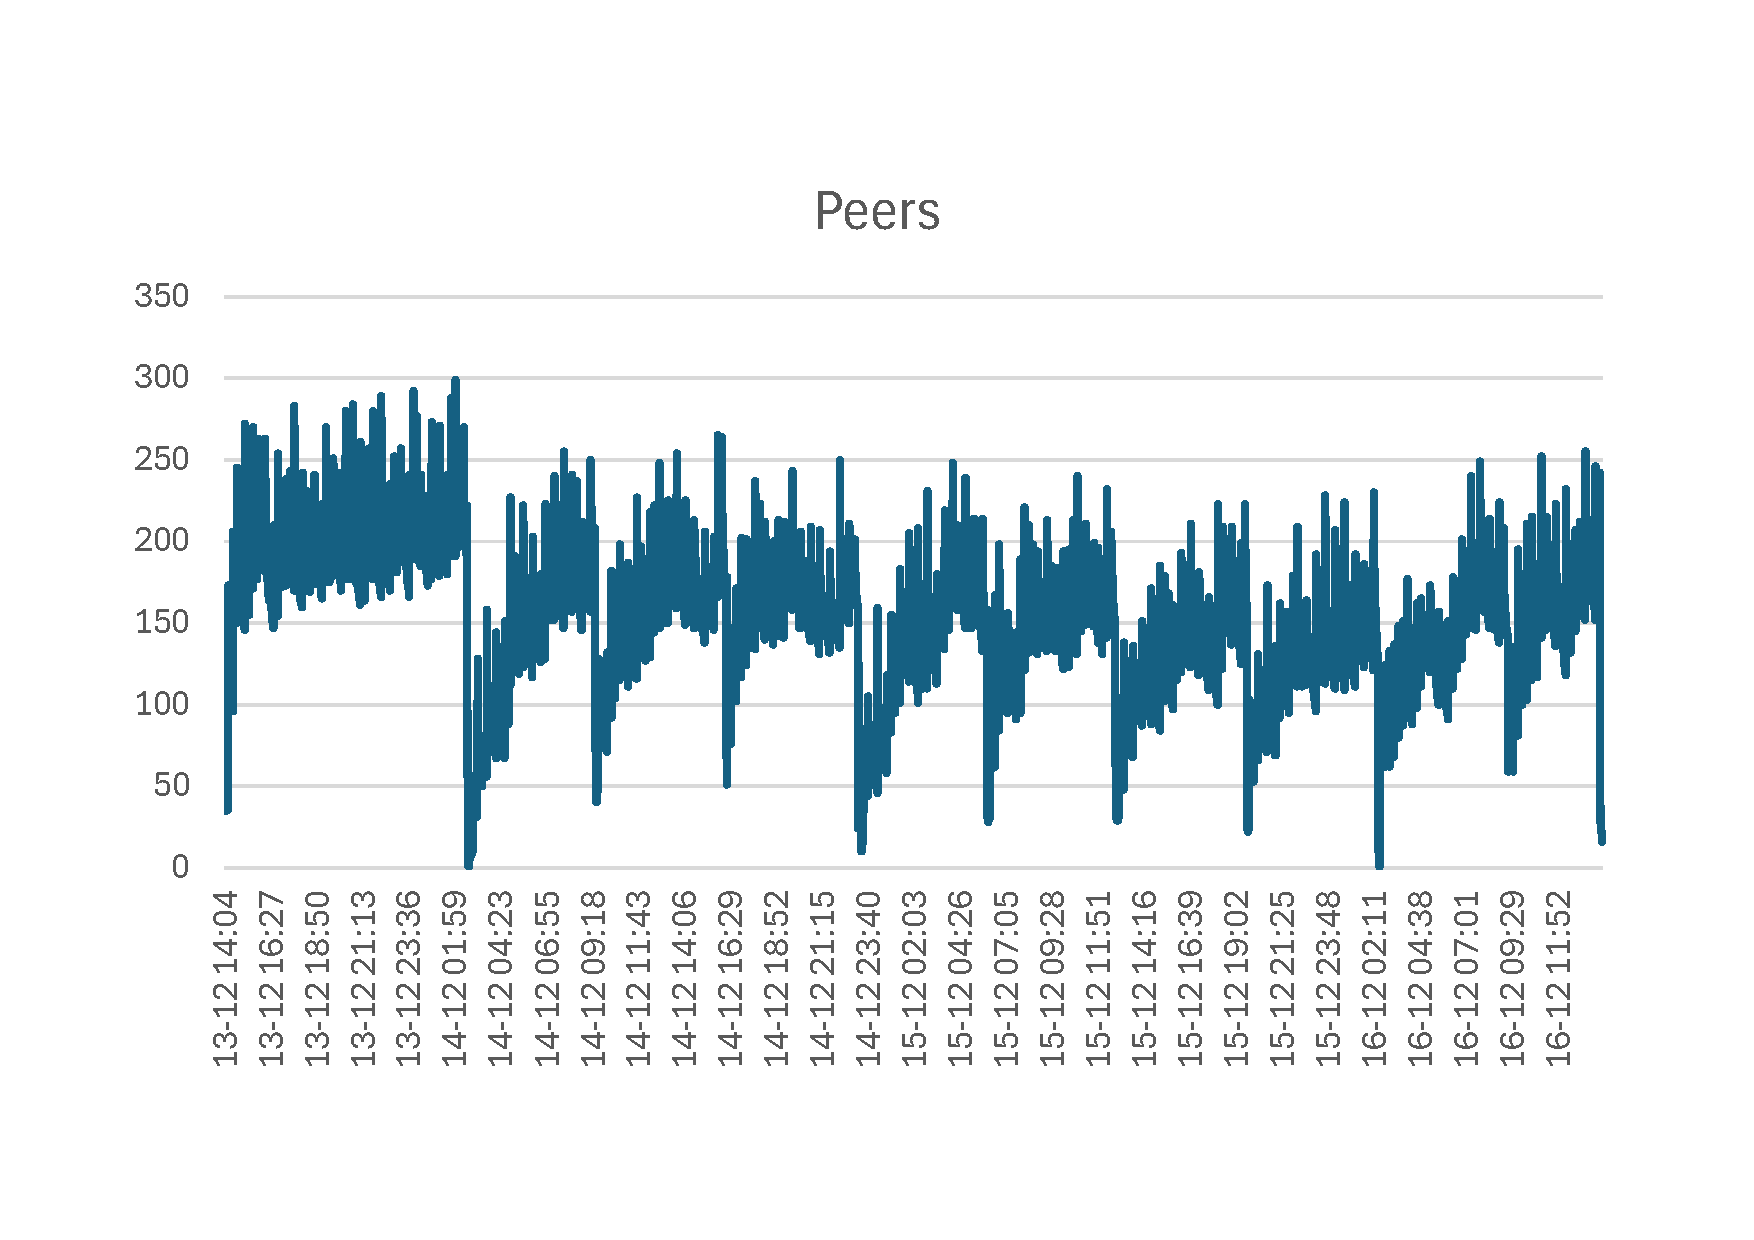
\includegraphics[width=\linewidth]{figures/conPeer2}
    \caption{The number of peers our node was connected to over the time of the experiment.
    Data points are collected every minute and the average amount of peers connected is 148.}
    \label{fig:peersconnected}
\end{figure*}
Throughout the experiment, we kept track of the number of peers our node was connected to.
The number of connected peers is shown in~\autoref{fig:peersconnected}.
Our node was connected to at most 300 peers at once, and the average was 148.
Over the course of the experiment, the number of connected peers fluctuated a lot but would continually rise for the first 12 hours.
Then it would heavily drop and rise again.
This pattern would repeat, but after the first drop it would then drop consistently every 7 hours instead.


\subsection{Deanonymization}\label{subsec:deanonymization}


\begin{table}[]
    \centering
    \caption{Distribution of nodes into the four different categories}
    \begin{tabular}{|l|l|l|}
        \hline
        & \textbf{Nodes} & \textbf{Distribution} \\ \hline
        \textbf{Deanonymized validators} & 513            & 42.93                 \\ \hline
        \textbf{64 subnets}              & 71             & 5.94                  \\ \hline
        \textbf{No validators}           & 0              & 0                     \\ \hline
        \textbf{Rest}                    & 611            & 51.13                 \\ \hline
    \end{tabular}
    \label{tab:distribution}
\end{table}


Deanonymized validators = 493,551

IPs collected = 1183

Average connected = 148

Nodes with validators = 513

\subsection{Validator Distribution}\label{subsec:validator-distribution}
\begin{figure*}[!ht]
    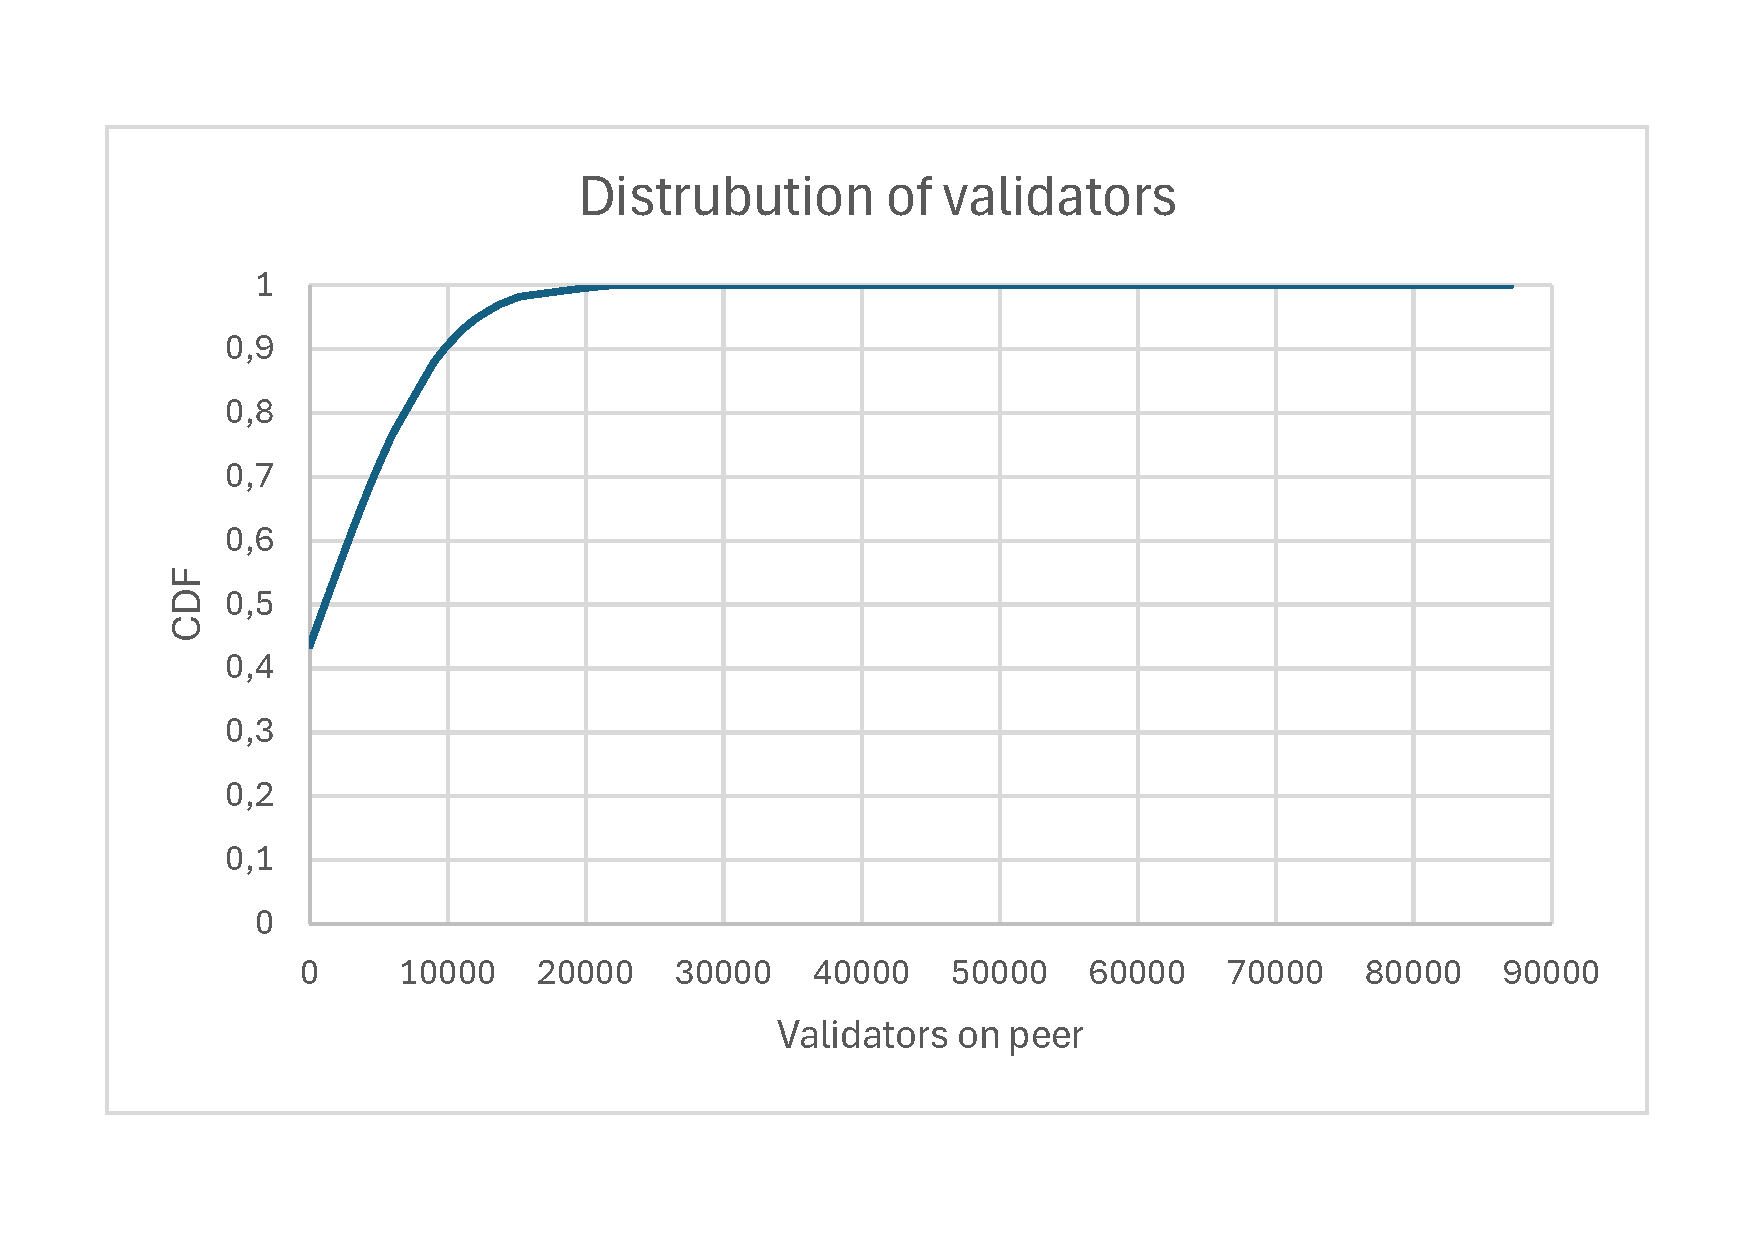
\includegraphics[width=\linewidth]{figures/cdf}
    \caption{The cdf showing the distribution of validators on each peer}
    \label{fig:validatorsonpeers}
\end{figure*}